il punto critico del sistema � il db e principalmente le op di scrittura 

abbiamo fatto uno script per testare le performance in scrittura e abbiamo cercato di capire come ottimizzare il db per le scritture

tre config di sharding
1 shard
2 shard id
2 shard hashed

parlare del balancer
dei lock di scrittura


come abbiamo eseguito i test:

3 VM 512mb ram, 1,2 ghz
1. mongos+config
2. mongod s1
3. mongod s2

media su 3 run

\begin{figure}[h]
\centering
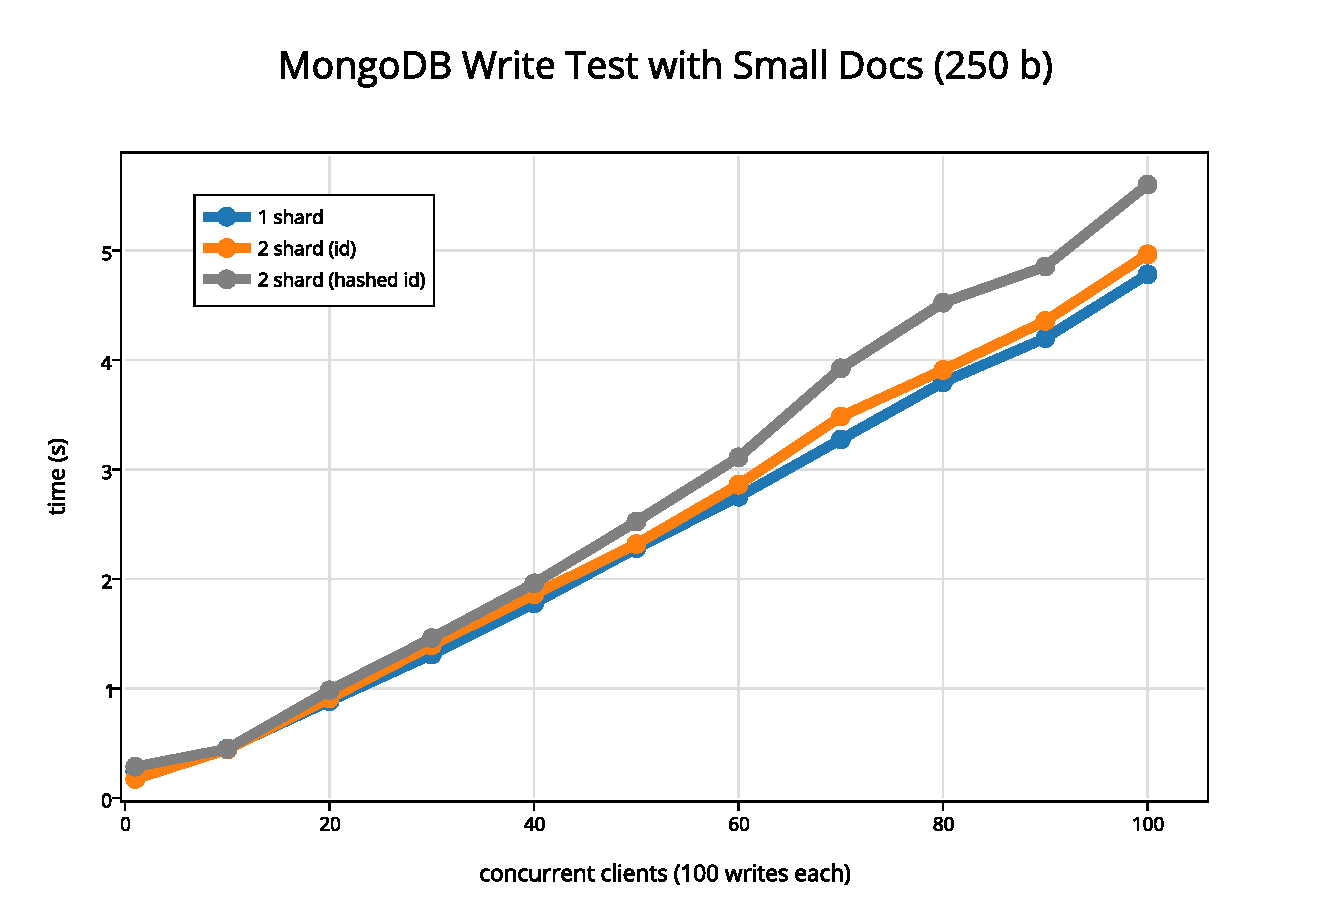
\includegraphics[width=1.0\linewidth]{./img/mongodb_write_test_with_small_docs_250_b}
\caption[small]{small}
\label{fig:benchmark-small}
\end{figure}

\begin{figure}[h]
\centering
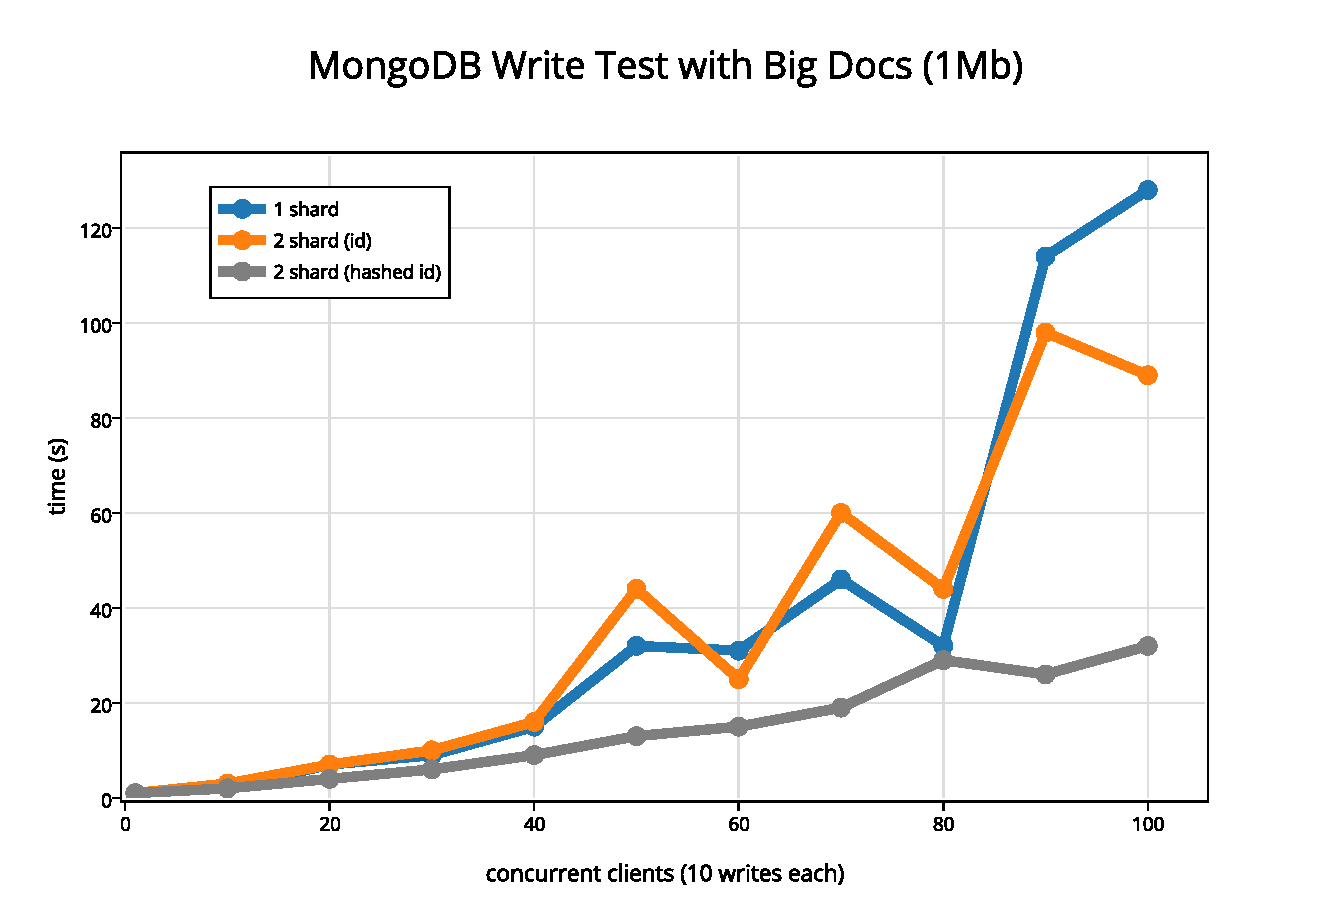
\includegraphics[width=1.0\linewidth]{./img/mongodb_write_test_with_big_docs_1mb}
\caption[big]{big}
\label{fig:benchmark-big}
\end{figure}

%problemi con i benchmark
%- dipendi dalla rete su cui sei
%- nostro client fatto con node - perch� non l'abbiamo usato
%- 2 parole sul tool che abbiamo usato
%- come sono stati fatti i benchmark
%- specifiche del sistema VM, ram, hdd, ...
%- risultati ottenuti


%non ha senso testare mole (server) per la parte rabbit (spiegare)
%il vero collo di bottiglia � il db
%abbiamo testato con configurazioni di db differenti

% parlare dei casini con le chiavi di shard


%conclusioni
%- la coda dei denormalizzatori rompe tra un test e l'altro (coda lunga async)

%problema bench su stessa macchina del server
%    v
%configuraz con vms 
%    v
%bench macchina fisica diversa
%    v
%shard key / ulimit(?)S
%    v





%strano comportamento: no denorm, gli dici di fare 10000 insert e trovi %10499[esatti] doc...
%--> motivo query su sources + insert in whispers #fail mi sa...

%con la nuova chiave lo sharding � sbilanciato 93% / 7%

%i write lock non sembrano avere drammi
%che sia la memoria?


% muore il socket sul benchmark

